
An open quantum system is a quantum-mechanical system that interacts with an external quantum system, which is known as the environment or a \textit{bath}. First of all, to describe an open system and its evolution, it is necessary to introduce the concept of \textit{mixed state}. 

\section{Mixed states}

A mixed state can be seen as an ensemble of quantum states in which each of them has an associated probability:
\begin{align*}
    \ket{\psi} ~~\text{pure state} \quad \longrightarrow \quad \left( \ket{\psi_\alpha}, p_\alpha \right) ~~\text{mixed state with} ~~\sum_\alpha p_\alpha = 1. 
\end{align*}
The states $\ket{\psi_\alpha}$ do not interfere, while the $p_\alpha$ are classical probabilities.

\subsubsection{Ensemble average and density operator}
The ensemble average of an operator $O$ on a mixed state is given by 
\begin{align*}
    \langle O \rangle_\text{ensemble} &\equiv \sum_\alpha p_\alpha \bra{\psi_\alpha} O \ket{\psi_\alpha} = \sum_\alpha p_\alpha \text{Tr}[ \, O \, \ket{\psi_\alpha} \bra{\psi_\alpha} \,] = \\
    &= \text{Tr} \left[ O \left( \sum_\alpha p_\alpha \ket{\psi_\alpha} \bra{\psi_\alpha} \right) \right] \equiv \text{Tr}[O \rho],
\end{align*}
where in the last line the \textit{density operator} (matrix) is introduced:
\begin{equation}
    \rho = \sum_\alpha p_\alpha \ket{\psi_\alpha} \bra{\psi_\alpha}. 
\end{equation}
The operator $\rho$ contains all the information about the system which is investigated. \\
The main properties of the density matrix are:
\begin{enumerate}
    \item Each element is positive (``$\rho \geq 0$"), which means that $\forall \ket{\phi}, ~\bra{\phi} \rho \ket{\phi} \geq 0$
    \begin{align*}
        & \implies \rho ~\text{is Hermitian} ~~ \rho = \rho^\dagger, \\
        & \implies \rho ~\text{can be diagonalized}, \\
        & \implies \text{Spec}(\rho) \geq 0. 
    \end{align*}
    \item Its trace is normalized to 1: i.e. Tr$[\rho] = 1$. 
    \item It represents the mixing of states and this does not produce interference; indeed, consider two matrix operators $\rho_1$ and $\rho_2$ and define 
    \begin{align*}
        \rho_+ = \frac{1}{2} \rho_1 + \frac{1}{2} \rho_2;
    \end{align*}
    for a given state $\ket{\phi}$, one can introduce 
    \begin{align*}
        P_1 &\equiv \text{Tr}[\ket{\phi}\bra{\phi} \rho_1] = \bra{\phi} \rho_1 \ket{\phi} \\
        P_2 &\equiv \text{Tr}[\ket{\phi}\bra{\phi} \rho_2] = \bra{\phi} \rho_2 \ket{\phi} \\
        P_+ &\equiv \text{Tr}[\ket{\phi}\bra{\phi} \rho_+] = \bra{\phi} \rho_+ \ket{\phi} = \\
        &= \frac{1}{2} \bra{\phi} \rho_1 \ket{\phi} + \frac{1}{2} \bra{\phi} \rho_2 \ket{\phi} = \frac{P_1 + P_2}{2}. 
    \end{align*}
    The probability of having $\ket{\phi}$ from the sum of the two mixtures is given by the sum of the probabilities in $\rho_1$ and $\rho_2$. 
\end{enumerate}

\subsection{Quantifier of the determinism}
Two quantities can be introduced to described how much a state is pure or mixed:
\begin{itemize}
    \item \textit{Purity}: 
    \begin{equation}
        \label{eq:purity}
        \mathcal{P} = \text{Tr}[\rho^2] \qquad \text{with} \qquad \frac{1}{\text{dim}_S} \leq \text{Tr}[\rho^2] \leq 1
    \end{equation}
    and $\mathcal{P} = 1$ indicates a pure state. 
    \item \textit{Entropy}
    \begin{equation}
        \label{eq:entropy}
        \mathcal{S} = -\text{Tr}[\rho \log \rho] \qquad \text{with} \qquad 0 \leq \mathcal{S} \leq \log{(\text{dim}_S)}
    \end{equation}
    and $\mathcal{S} = 0$ indicates a pure state. The entropy increases when the one loses information about the system. Moreover, it is important to remember that the logarithm of an operator is define according to the Taylor expansion. 
\end{itemize}

\begin{tcolorbox} [breakable, enhanced]
\textbf{Discrete mixing of states} \\
Consider a mixture of two states $\ket{\psi_1}$ and $\ket{\psi_2}$ on the surface of the Bloch sphere, as represented in figure \ref{fig:mix_states1}, and in the $xz$ plane:
\begin{align*}
    \ket{\psi_1} = \begin{pmatrix} \cos{\theta} \\ \sin{\theta} \end{pmatrix} \qquad \text{and} \qquad \ket{\psi_2} = \begin{pmatrix} \cos{\theta} \\ -\sin{\theta} \end{pmatrix}
\end{align*}
It is straightforward to see that 
\begin{align*}
    \langle \sigma^x \rangle_{\psi_1} &= \sin{(2 \theta)} \qquad \langle \sigma^x \rangle_{\psi_2} = -\sin{(2 \theta)} \\  
    \langle \sigma^z \rangle_{\psi_1} &= \cos{(2 \theta)} \qquad \langle \sigma^z \rangle_{\psi_2} = \cos{(2 \theta)}
\end{align*}
and that $\langle \sigma^y \rangle_{\psi_1} = \langle \sigma^y \rangle_{\psi_2} = 0$. The density operator is 
\begin{align*}
    \rho = \frac{1}{2} \ket{\psi_1}\bra{\psi_1} + \frac{1}{2} \ket{\psi_2}\bra{\psi_2} = \begin{pmatrix} \cos^2{\theta} & 0 \\ 0 & \sin^2{\theta} \end{pmatrix} = \cos^2{\theta} \ket{0}\bra{0} + \sin^2{\theta} \ket{1}\bra{1},
\end{align*}
with Tr$[\rho]$ = 1. Moreover, 
\begin{align*}
    \text{Tr}[\sigma^x \rho] = \langle \sigma^x \rangle = 0 \qquad \text{and} \qquad \text{Tr}[\sigma^z \rho] = \langle \sigma^z \rangle = \cos{(2\theta)}. 
\end{align*}
The purity of $\rho$ is evaluated as in (\ref{eq:purity}): 
\begin{align*}
    \text{Tr}[\rho^2] = \cos^4 \theta + \sin^4 \theta = \frac{1}{2} (1 + \cos^2{(2 \theta)}) &= 1 ~~\text{if}~~ 2\theta = 0 ~~\text{or}~~ 2\theta = \pi \\
    &= 0 ~~\text{if}~~ 2 \theta = \pi/2
\end{align*}
\end{tcolorbox}

\begin{figure}[H]
\centering
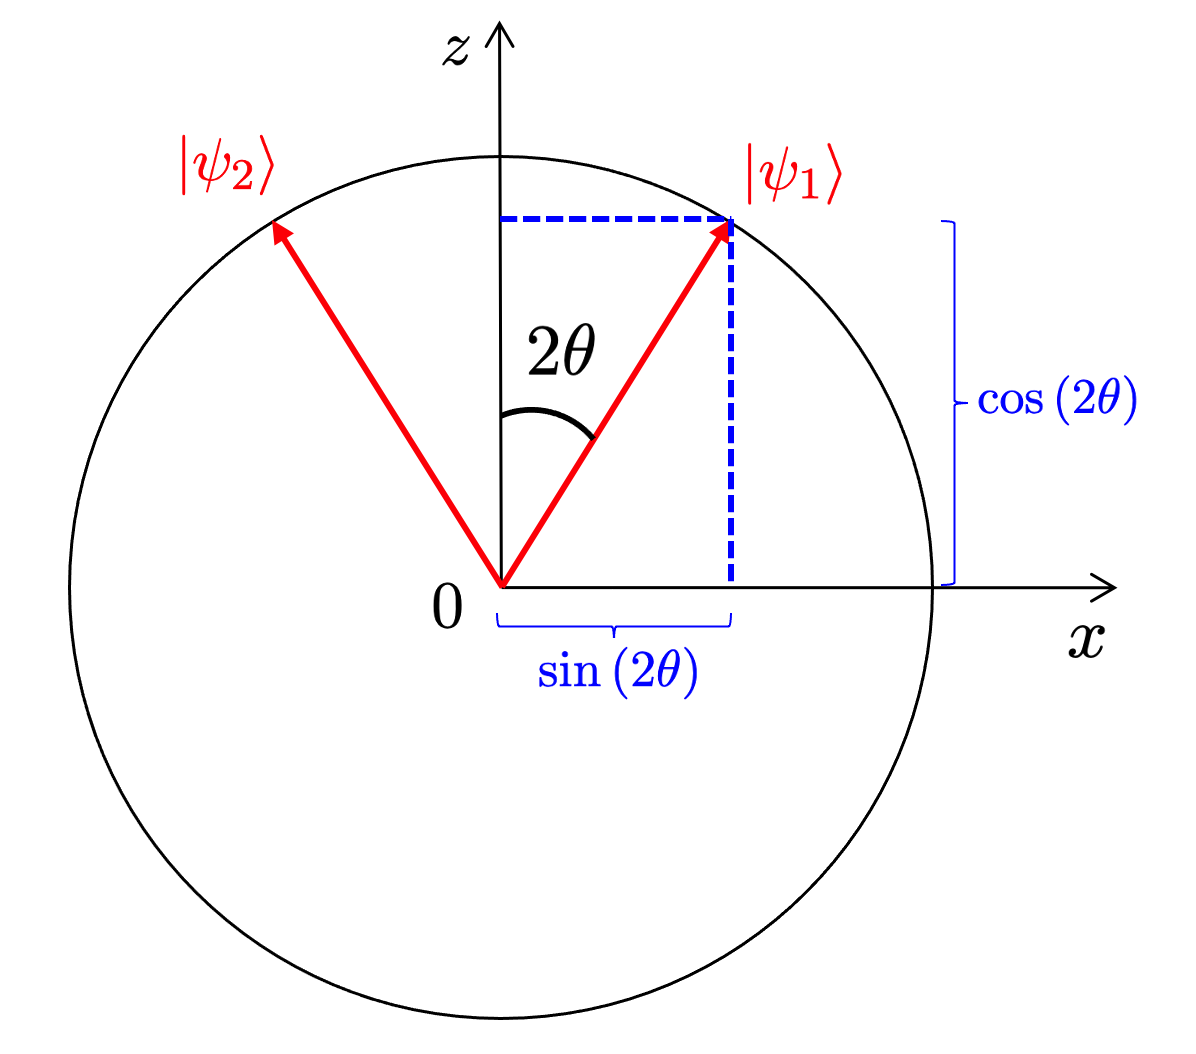
\includegraphics[width=0.48\linewidth]{images/Mixing_states_1.png}
    \caption{Discrete mixing of states on the surface of a Bloch sphere; only the $x-z$ plane of it is represented in this figure.}
    \label{fig:mix_states1}
\end{figure}

\begin{tcolorbox} [breakable, enhanced]
\textbf{Continuous mixing of states} \\
Consider a continuous mixing of states which are on the surface of the Bloch sphere, as shown in figure \ref{fig:mix_states2}; one of them is
\begin{align*}
    \ket{\psi(\theta,\varphi)} = \begin{pmatrix} \cos{\theta} \\ e^{i \varphi} \sin{\theta} \end{pmatrix}. 
\end{align*}
The density operator is 
\begin{align*}
    \rho &= \int \ket{\psi(\theta,\varphi)} \bra{\psi(\theta,\varphi)} \, dP(\varphi) = \\
    &= \int \ket{\psi(\theta,\varphi)} \bra{\psi(\theta,\varphi)} \, \frac{d \varphi}{2 \pi} = \\
    &= \int \begin{pmatrix} \cos^2{\theta} & e^{i \varphi} \cos{\theta} \sin{\theta} \\ \text{h.c.} & \sin^2{\theta} \end{pmatrix} \frac{d \varphi}{2 \pi} = \\
    &= \begin{pmatrix} \cos^2{\theta} & 0 \\ 0 & \sin^2{\theta} \end{pmatrix} 
\end{align*}
\end{tcolorbox}

\begin{figure}[H]
\centering
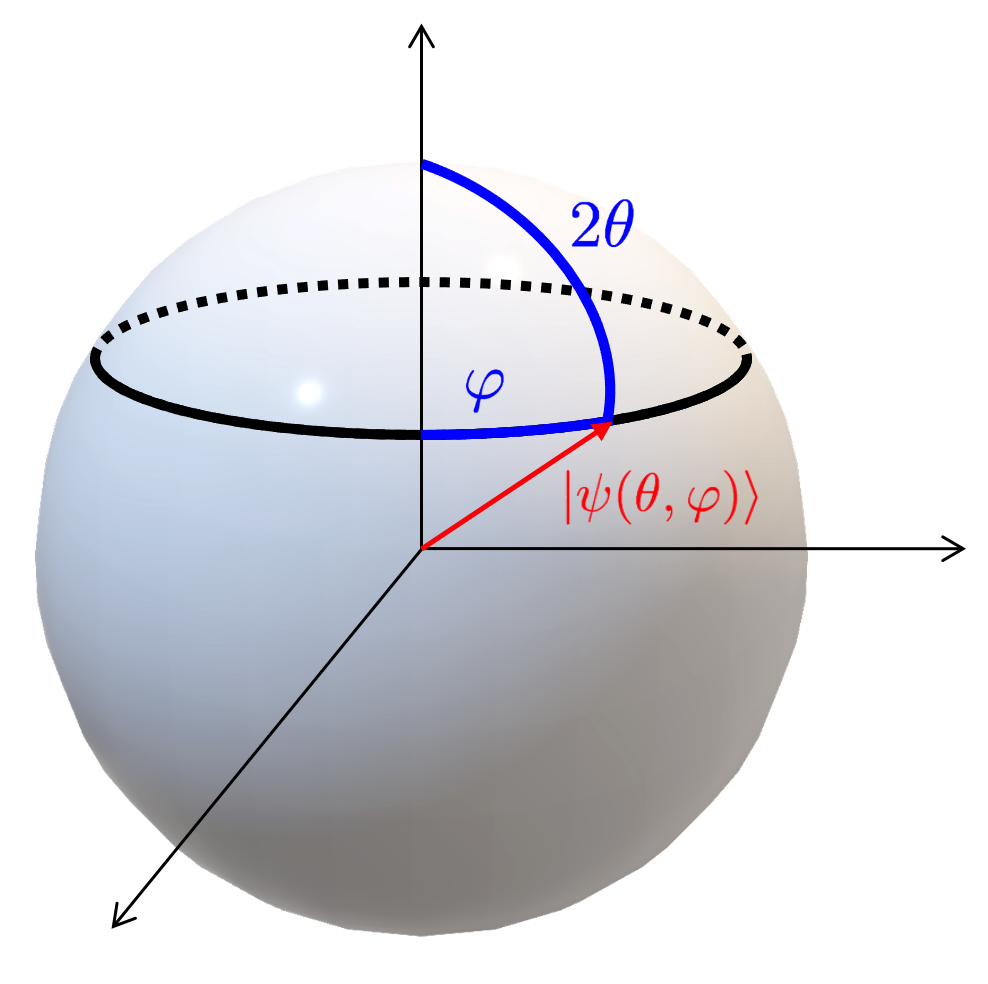
\includegraphics[width=0.45\linewidth]{images/Mixing_states_2.png}
    \caption{Continuous mixing of states on the surface of a Bloch sphere; for fixed values of $\theta$ and $\varphi$, the states $\ket{\psi(\theta,\varphi)}$ lie on a circumference.}
    \label{fig:mix_states2}
\end{figure}

\subsection{Reduced density operator}

In general, the interactions between the quantum system and the environment significantly change the dynamics of the system, therefore it is useful to develop a theoretical framework for treating them and for obtaining an accurate description of the dynamics of the system. Consider a bi-partition of a system into subsystem $A$ and subsystem $B$ which are associated to two Hilbert spaces with dimensions dim$_A$ and dim$_B$ and with sets of orthonormal bases $\ket{a_i}$ ($i = 1, ...,$ dim$_A$) and $\ket{b_j}$ ($j = 1, ...,$ dim$_B$), respectively. A generic element of the total system can be always written as 
\begin{align*}
    \ket{ab} = \sum_{i = 1}^{\text{dim}_A} \sum_{j = 1}^{\text{dim}_B} C_{ij} \ket{a_i}_A \otimes \ket{b_j}_B,
\end{align*}
where because of normalization 
\begin{align*}
    \sum_{i = 1}^{\text{dim}_A} \sum_{j = 1}^{\text{dim}_B} \abs{C_{ij}}^2 = 1.
\end{align*}
Consider now an observable of the full system $O_{AB} = O_A \otimes \mathbb{1}_B$ and evaluate the ensemble average:  
\begin{align*}
    \langle O_{AB} \rangle &= \text{Tr}[\left( O_A \otimes \mathbb{1}_B \right) \rho_{AB}] = \\
    &= \sum_a \sum_b (\bra{a}_A \otimes \bra{b}_B) \, \left[O_A \otimes \mathbb{1}_B \rho_{AB}\right] \, ( \ket{a}_A \otimes \ket{b}_B )= \\
    &= \sum_a \bra{a}_A O_A \left( \sum_b \bra{b}_B \rho_{AB} \ket{b}_B \right) \ket{a}_A = \\
    &= \sum_a \bra{a}_A O_A \rho_A \ket{a}_A = \\
    &= \text{Tr}[O_A \rho_A],
\end{align*}
where in the forth line the matrix operator $\rho_A$ is introduced
\begin{align}
    \rho_A = \sum_b \bra{b}_B \rho_{AB} \ket{b}_B = \text{Tr}_B[\rho_{AB}]
    \label{eq:rhoA}
\end{align}
and it is called \textit{reduced density operator} (or \emph{partial trace}) over system A. 
An analogous definition of $\rho_B$ can be obtained considering the observable $O_{AB} = \mathbb{1}_A \otimes O_B$:
\begin{align}
    \rho_B = \sum_a \bra{a}_A \rho_{AB} \ket{a}_A = \text{Tr}_A[\rho_{AB}].
    \label{eq:rhoB}
\end{align}
From these results, one can conclude that having $\rho_{AB}$ allows to obtain $\rho_A$ and $\rho_B$, but knowing $\rho_A$ and $\rho_B$ separately is not enough to reconstruct $\rho_{AB}$. Some examples relative to the evaluation of these quantities are given in the following. 

\begin{tcolorbox} [breakable, enhanced]
\textbf{Quantum correlated (entangled) state} \\ 
Consider the state $\ket{\Phi}$ and its associated density matrix
\begin{align*}
    \ket{\Phi} = \frac{1}{\sqrt{2}} \left( \ket{0 0 } + \ket{1 1} \right) \qquad \longrightarrow \qquad \rho = \frac{1}{2} \begin{pmatrix} 1 & 0 & 0 & 1 \\ 0 & 0 & 0 & 0 \\ 0 & 0 & 0 & 0 \\ 1 & 0 & 0 & 1 \end{pmatrix}.
\end{align*}
The reduced density operator $\rho_A$ is 
\begin{align*}
    \rho_A  = \frac{1}{2} \begin{pmatrix} 1 & 0 \\ 0 & 1 \end{pmatrix} = \frac{\mathbb{1}}{2}.
\end{align*}
\end{tcolorbox}

\begin{tcolorbox} [breakable, enhanced]
\textbf{Classical correlated state} \\ 
Consider the density matrix
\begin{align*}
    \rho = \frac{1}{2} \left( \ket{00} \bra{00} + \ket{11} \bra{11} \right) = \frac{1}{2} \begin{pmatrix} 1 & 0 & 0 & 0 \\ 0 & 0 & 0 & 0 \\ 0 & 0 & 0 & 0 \\ 0 & 0 & 0 & 1 \end{pmatrix}.
\end{align*}
Note that this state is not quantum entangled. The reduced density operator $\rho_A$ is 
\begin{align*}
    \rho_A = \frac{1}{2} \begin{pmatrix} 1 & 0 \\ 0 & 1 \end{pmatrix} = \frac{\mathbb{1}}{2}
\end{align*}
and it is the same obtained in the previous example despite the total density matrix is different.
\end{tcolorbox}

\begin{tcolorbox} [breakable, enhanced]
\textbf{Uncorrelated state} \\ 
Consider the density matrix
\begin{align*}
    \rho = \frac{1}{4} \left( \ket{00} \bra{00} + \ket{01} \bra{01} + \ket{10} \bra{10} +\ket{11} \bra{11} \right) = \frac{1}{4} \begin{pmatrix} 1 & 0 & 0 & 0 \\ 0 & 1 & 0 & 0 \\ 0 & 0 & 1 & 0 \\ 0 & 0 & 0 & 1 \end{pmatrix}.
\end{align*}
The reduced density operator $\rho_A$ is 
\begin{align*}
    \rho_A = \frac{1}{2} \begin{pmatrix} 1 & 0 \\ 0 & 1 \end{pmatrix} = \frac{\mathbb{1}}{2}
\end{align*}
which is equal to ones obtained previously. 
\end{tcolorbox}

From these examples, one can conclude that the partial trace hides (or deletes) the correlations between the elements of the subsystem $A$ and the elements of the subsystem $B$. \\


\section{System dynamics}
\label{sec:ME}

\subsection{Evolution of a closed quantum system}

For a given quantum system, the density operator at the initial and at the final instants of time are
\begin{align*}
    \rho_0 = \sum_\alpha p_\alpha \ket{\psi_\alpha} \bra{\psi_\alpha} \qquad \text{and} \qquad \rho(t) = \sum_\alpha p_\alpha \ket{\psi_\alpha(t)} \bra{\psi_\alpha(t)}.
\end{align*}
It is important to notice that every member evolves by itself (there is no interference) and therefore the probabilities $p_\alpha$ are static ($\dot{p}_\alpha = 0$). 
The evolution of the system is described by $\dot{\rho}(t)$ and from the previous relation 
\begin{align*}
    \dot{\rho}(t) &= \sum_\alpha p_\alpha \left( \ket{\dot{\psi}_\alpha(t)} \bra{\psi_\alpha(t)} + \ket{\psi_\alpha(t)} \bra{\dot{\psi}_\alpha(t)} \right) = \\
    &= \sum_\alpha p_\alpha \left( -\frac{i}{\hbar} H \ket{\psi_\alpha(t)} \bra{\psi_\alpha(t)} + \frac{i}{\hbar} \ket{\psi_\alpha(t)} \bra{\psi_\alpha(t)} H \right) = \\
    &= -\frac{i}{\hbar} H \left( \sum_\alpha p_\alpha \ket{\psi_\alpha(t)} \bra{\psi_\alpha(t)} \right) + \frac{i}{\hbar} \left( \sum_\alpha p_\alpha \ket{\psi_\alpha(t)} \bra{\psi_\alpha(t)} \right) H = \\
    &= \frac{i}{\hbar} [\rho,H].
\end{align*}
Some considerations about this result can be done:
\begin{itemize}
    \item The relation 
    \begin{equation}
        \label{eq:evol_rho}
        \dot{\rho}(t) = \frac{i}{\hbar} [\rho,H]
    \end{equation}
    is similar to the evolution equation for operators in the Heisenberg picture but with a different sign; this comes from the fact that the dynamics of the system is studied in the Schr\"odinger picture (the statevectors are functions of time). 
    \item If the mixture is made of eigenstates of $H$, it does not evolve in time (stationary system) because the commutator in (\ref{eq:evol_rho}) is null. 
\end{itemize}

\subsection{Evolution of an open quantum system}

In general, to describe the dynamics of an open quantum system, one needs to track the evolution of both the system and the bath together, but there are particular situations in which is possible to describe only the dynamics of the system without its coupling with the bath. This type of dynamics is called \textit{Born-Markovian dynamics} and it is based on the fact that, under certain requirements, the considered bath loses immediately memory of his interaction with the quantum system. This situation is schematize in the figure \ref{fig:sys_bath}. From the latter, it is possible to notice that:
\begin{itemize}
    \item the information proceeds only in one direction, from the system to the bath, it never comes back to the system;
    \item the bath needs to have an environment where to put acquired information, which is lost immediately.
\end{itemize}

\begin{figure}[H]
\centering
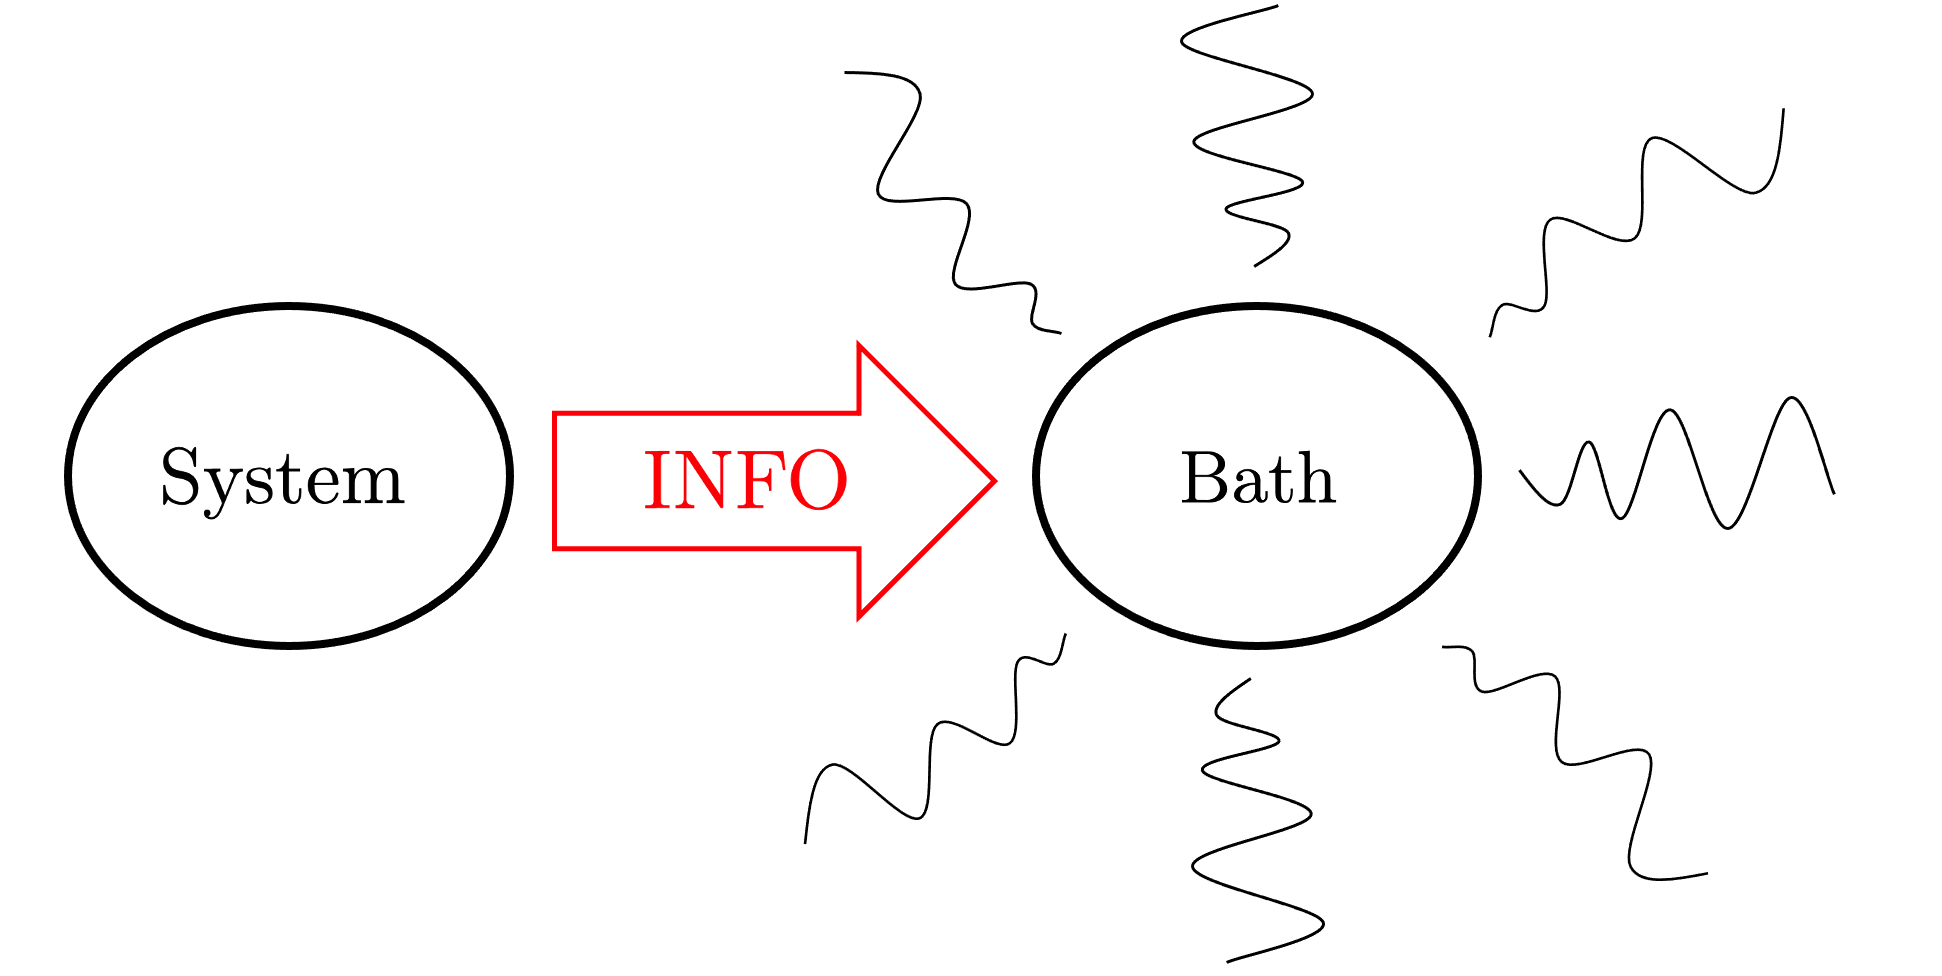
\includegraphics[width=0.68\linewidth]{images/System_and_Bath.png}
    \caption{System and bath in Born-Markovian dynamics; the information proceeds only in one direction, from the system to the bath, which immediately loses it.}
    \label{fig:sys_bath}
\end{figure}
Two physical requirements are necessary to realise this situation: 
\begin{enumerate}
    \item The bath has to be fast. If the system is described by the total Hamiltonian 
    \begin{align}
        H_\text{tot} = H_S + H_B + H_\text{int}
        \label{eq:HamLind}
    \end{align}
    and if each term is associate to a typical time $\tau_S$, $\tau_B$ and $\tau_\text{int}$, then the timescale separation must be
    \begin{align*}
        \tau_B \ll \tau_S  \lesssim \tau_\text{int}. 
    \end{align*}
    The first relation is required for the Born-Markovian dynamics, while the second one is useful for the quantum applications and technologies of the open system. 
    \item The bath has to be large. This means that dim$_S$ $\ll$ dim$_B$, since the bath must have space to store and forget information about the system. 
\end{enumerate}

In this framework, it is possible to describe the evolution of the density matrix for an open system described by a density matrix $\rho$ and with Hamiltonian $H$. The latter follows the \textit{Lindblad Master Equation}:
\begin{equation}
    \dot{\rho} = \frac{i}{\hbar} [\rho,H] + \sum_j \gamma_j \left( L_j \, \rho \,  L_j^\dagger - \frac{1}{2} \Bigl\{ L_j^\dagger L_j, \, \rho \Bigr\} \right),
    \label{eq:Lindblad}
\end{equation}
where:
\begin{itemize}
    \item $\rho$ and $H$ are operators associated only to the system ($H = H_S$ and $\rho = \rho_S$); 
    \item the first term in the right hand side describes the evolution of a closed quantum system, while the second term is associated to the coupling between the bath and the considered system;
    \item $\gamma_j$ is positive and has the dimension of s$^{-1}$, therefore it can be associated to a frequency (for instance, a rate of decay or a lifetime);
    \item $L_j$ are commonly called the \textit{Lindblad} or \textit{jump operators} of the system. 
\end{itemize}
The explicit expressions for $\gamma_\alpha$ and $L_\alpha$ can be obtained from the microscopic derivation of (\ref{eq:Lindblad}) which is presented in the following section. 

\subsection{Microscopic derivation of the Lindblad Master equation}

The starting point is the time-independent Hamiltonian in (\ref{eq:HamLind}) in which 
\begin{align*}
    H_S &= H_S \otimes \mathbb{1}_B, \\
    H_B &= \mathbb{1}_S \otimes H_B, \\
    H_\text{int} &= \sum_\alpha S_\alpha \otimes B_\alpha = \sum_\beta S_\beta^\dagger \otimes B_\beta^\dagger.
\end{align*}
The transformation 
\begin{align*}
    U(t) = \exp{\frac{i}{\hbar}t(H_S + H_B)}
\end{align*}
introduces $H'$ according to relation (\ref{eq:transfH}): 
\begin{align*}
    H'(t) &= U(t) H U^\dagger(t) - i \hbar U(t) \dot{U}^\dagger(t) = \\
    &= \exp{\frac{i}{\hbar}t(H_S + H_B)} (H_S + H_B + H_\text{int}) \exp{-\frac{i}{\hbar}t(H_S + H_B)} ~+ \\
    & \qquad - \exp{\frac{i}{\hbar}t(H_S + H_B)} (H_S + H_B) \exp{-\frac{i}{\hbar}t(H_S + H_B)} = \\
    &= \exp{\frac{i}{\hbar}t(H_S + H_B)} H_\text{int} \exp{-\frac{i}{\hbar}t(H_S + H_B)} = \\
    &= U(t) H_\text{int} U^\dagger(t),
\end{align*}
while $\rho(t) = \rho_{SB}(t)$ becomes
\begin{align*}
     \rho_{SB}'(t) = U(t) 
{\rho}_{SB}(t) U^\dagger(t).
\end{align*}
Therefore, equation (\ref{eq:evol_rho}) can be rewritten as 
\begin{align}
    \dot{\rho}'_{SB}(t) = \frac{i}{\hbar} [{\rho}'_{SB}(t), H'(t)].
    \label{eq:new_rho}
\end{align}
By integrating in time both sides of this relation, one obtains
\begin{align*}
    \rho_{SB}'(t) = \rho_{SB}'(0) + \frac{i}{\hbar} \int_0^t dt'[\rho_{SB}'(t'), H'(t')] 
\end{align*}
and by inserting this result in (\ref{eq:new_rho}) one can write an integro-differential equation:
\begin{align*}
    \dot{\rho}'_{SB}(t) = \frac{i}{\hbar} [{\rho}'_{SB}(0), H'(t)] - \frac{1}{\hbar^2} \int_0^t dt' \, [[\rho_{SB}'(t'), H'(t')], H'(t)] \equiv \triangle + \square.
\end{align*}
In the latter expression, the symbols $\triangle$ and $\square$ are introduced in order to indicate the commutator and the integral terms. \\
Now the trace over the bath density matrix of this equation is applied on the left and on the right; in order to develop the calculations, the contributions are studied separately. In particular:
\begin{itemize}
    \item In order to evaluate $\text{Tr}_B [ \triangle]$ the \textit{Born approximation} is used. The latter states that 
    \begin{align}
        \rho_{SB}(t) &= \rho_S(t) \otimes \rho_B(0), \\
        \rho'_{SB}(t) &= \rho'_S(t) \otimes \rho'_B(0) = \rho'_S(t) \otimes \rho_B(0).
    \end{align}
    and it means that the states of the system and of the bath are not correlated and that the latter does not evolve in time (stationary bath). Moreover, the following redefinitions of the parts of $H$ are considered: 
    \begin{align*}
        H_S \quad \longrightarrow \quad &H_S + \sum_\alpha S_\alpha \langle B_\alpha \rangle_B \\
        H_\text{int} \quad \longrightarrow \quad & H_\text{int} - \sum_\alpha S_\alpha \langle B_\alpha \rangle_B = \sum_\alpha S_\alpha \otimes \left(B_\alpha - \langle B_\alpha \rangle_B\right)
    \end{align*}
    Therefore
\begin{align*}
    \text{Tr}_B [\triangle] &= \frac{i}{\hbar} \text{Tr}_B \big( [\rho'_S(0) \otimes \rho_B(0),H'(t)]  \big) = \\
    &= \frac{i}{\hbar} \text{Tr}_B \left( \left[ \rho'_S(0) \otimes \rho_B(0),\sum_\alpha S'_\alpha \otimes (B'_\alpha - \langle B'_\alpha \rangle_B) \right] \right) = \\
    &= \frac{i}{\hbar} \sum_\alpha [\rho'_S(0),S'_\alpha(t)] \, \text{Tr}_B \Big( \rho_B(0) \left( B'_\alpha(t) - \langle B'_\alpha \rangle_B \right)\Big) = \\
    &= \frac{i}{\hbar} \sum_\alpha [\rho'_S(0),S'_\alpha(t)] \Big( \text{Tr}_B \left( \rho_B(0) B'_\alpha(t) \right) - \text{Tr}_B \left( \rho_B(0) \langle B'_\alpha \rangle_B \right) \Big) = \\
    &= \frac{i}{\hbar} \sum_\alpha [\rho'_S(0), S'_\alpha(t)] \left(\langle B'_\alpha \rangle_B - \langle B'_\alpha \rangle_B \right) = 0.
\end{align*}
From the second to the third line, some properties of the tensor product and of the trace operator are exploited (see Appendix A).
\item Also to evaluate 
\begin{align*}
     \text{Tr}_B [\square] &= \text{Tr}_B \left(- \frac{1}{\hbar^2} \int_0^t dt'\, [[\rho_{SB}'(t'), H'(t')], H'(t)] \right) = \\
     &= - \frac{1}{\hbar^2} \int_0^t dt' \, \text{Tr}_B \left([[\rho_{SB}'(t'), H'(t')], H'(t)] \right) = \\
    &= \frac{1}{\hbar^2} \int_0^t dt' \, \text{Tr}_B \left([[H'(t'),\rho_{SB}'(t')], H'(t)] \right)
\end{align*}
the Born approximation is used. In addition, the following expressions for $H'(t')$ and $H'(t)$ are inserted
\begin{align*}
    H'(t') &= \sum_\alpha S'_\alpha(t') \otimes B'_\alpha(t') \\
    H'(t) &= \sum_\beta S'^\dagger_\beta(t) \otimes B'^\dagger_\beta(t),
\end{align*}
in order to obtain 
\begin{align*}
    \text{Tr}_B [\square] = \frac{1}{\hbar^2} \int_0^t dt'\sum_{\alpha, \beta} S'_\alpha(t') \rho'_S(t') S'^\dagger_\beta(t) \, \text{Tr}_B \left[  B'_\alpha(t') \rho_B(0) B'^\dagger_\beta(t) \right] +\text{other 3 parts}.
\end{align*}
The trace in the previous expression can be evaluated explicitly: 
\begin{align*}
    \text{Tr}_B \left[  B'_\alpha(t') \rho_B(0) B'^\dagger_\beta(t) \right] &= \text{Tr}_B \left[ \rho_B(0) B'_\alpha(t')  B'^\dagger_\beta(t) \right] = \\
    &= \text{Tr}_B \left[ \rho_B(0) e^{i H_B t/\hbar} B_\beta^\dagger e^{-i H_B t/\hbar} e^{i H_B t'/\hbar} B_\alpha e^{-i H_B t'/\hbar} \right] = \\
    &= \text{Tr}_B \left[ \rho_B(0) e^{i H_B (t-t')/\hbar} B_\beta^\dagger e^{-i H_B (t-t')/\hbar} B_\alpha \right] = \\
    &= \text{Tr}_B \left[ \rho_B(0) {B'}_\beta^{\dagger}(t-t') B_\alpha \right] = \\
    &= \langle {B'}_\beta^\dagger(t-t') B_\alpha \rangle_B \equiv G_{\alpha \beta} (t-t')
\end{align*}
and hence
\begin{align}
    \text{Tr}_B [\square] =& \frac{1}{\hbar^2} \int_0^t dt' \sum_{\alpha, \, \beta} \bigg( G_{\alpha \beta} (t-t') \left( S'_\alpha(t') \rho'_S(t') S'^\dagger_\beta(t) - {S'}_\beta^\dagger(t) S'_\alpha(t') \rho'_S(t') \right) + \nonumber\\
    &+ G_{ \beta \alpha} (t'-t) \left( {S'}_\beta^\dagger(t) \rho'_S(t') S'_\alpha(t') - \rho'_S(t') S'_\alpha(t') {S'}_\beta^\dagger(t) \right) \bigg).
    \label{eq:cos}
\end{align}
At this point, another approximation to evaluate $G_{\alpha \beta}$ and $G_{\beta \alpha}$ is introduced; it is the \textit{Markov approximation} according to which
\begin{align*}
    G_{\alpha \beta} (t-t') = G_{\alpha \beta}(0) \delta(t-t') \qquad \text{and} \qquad   G_{\beta \alpha} (t'-t) = G_{\beta \alpha}(0) \delta(t'-t).
\end{align*}
It means that the time correlations of the bath decays are so fast that they can be approximated by a Dirac-$\delta$ function. Therefore
\begin{align*}
    \text{Tr}_B [\square] =& \frac{1}{\hbar^2} \sum_{\alpha, \, \beta} \bigg( G_{\alpha \beta} (0) \left( S'_\alpha(t) \rho'_S(t) S'_\beta(t) - {S'}_\beta^\dagger(t) S'_\alpha(t) \rho'_S(t) \right) ~+ \\
    &+ G_{ \beta \alpha} (0) \left( {S'}_\beta^\dagger(t) \rho'_S(t) S'_\alpha(t) - \rho'_S(t) S'_\alpha(t) {S'}_\beta^\dagger(t) \right) \bigg).
\end{align*}
By noticing that 
\begin{align*}
    G_{\alpha \beta}(0) &= \langle {B'}_\beta^\dagger(0) B'_\alpha(0) \rangle_B = \langle B_\beta^\dagger(0) B_\alpha(0) \rangle_B \\
    G_{\beta \alpha}(0) &= \langle {B'}_\alpha^\dagger(0) B'_\beta(0) \rangle_B = \langle B_\alpha^\dagger(0) B_\beta(0) \rangle_B \\
    G_{\alpha \beta}(0) &= G_{\beta \alpha}(0),
\end{align*}
the final result is 
\begin{align*}
    \text{Tr}_B [\square] &= \frac{1}{\hbar^2} \sum_{\alpha, \,\beta}  G_{\alpha \beta} (0) \bigg( 2 S'_\alpha(t) \rho'_S(t) S'_\beta(t) - {S'}_\beta^\dagger(t) S'_\alpha(t) \rho'_S(t) ~+ \\
    & \qquad - \rho'_S(t) {S'}_\beta^\dagger(t) S'_\alpha(t)  \bigg) = \\
    &= \frac{1}{\hbar^2} \sum_{\alpha, \,\beta}  G_{\alpha \beta} (0) \bigg( 2 S'_\alpha(t) \rho'_S(t) S'_\beta(t) - \Bigl\{\rho'_S(t), {S'}_\beta^\dagger(t) S'_\alpha(t)\Bigr\} \bigg)
\end{align*}
\item The left-hand part in the Born approximation gives 
    \begin{align*}
        \text{Tr}_B \left[ \dot{\rho}'_{SB}(t) \right] &= \text{Tr}_B \left[ \dot{\rho}'_{S}(t)  \otimes \rho_B(0) \right] +  \text{Tr}_B \left[ {\rho}'_{S}(t)  \otimes \dot{\rho}_B(0) \right] = \\
        &= \text{Tr}_B \left[ \dot{\rho}'_{S}(t) \right] \text{Tr}_B \left[\rho_B(0) \right] + \text{Tr}_B \left[ {\rho}'_{S}(t) \right] \text{Tr}_B \left[ \dot{\rho}_B(0) \right] = \\
        &= \text{Tr}_B \left[ \dot{\rho}'_{S}(t) \right] = \dot{\rho}'_{S}(t),
    \end{align*}
    since 
    \begin{align*}
        \text{Tr}_B \left[\rho_B(0) \right] = 1 \qquad \text{and} \qquad \text{Tr}_B \left[ \dot{\rho}_B(0) \right] = 0. 
    \end{align*}
\end{itemize}
Using these results, one obtains 
\begin{align*}
    \dot{\rho}'_{S}(t) = \frac{1}{\hbar^2} \sum_{\alpha,\, \beta} G_{\alpha \beta} (0) \bigg( 2 S'_\alpha(t) \rho'_S(t) S'_\beta(t) - \Bigl\{\rho'_S(t), {S'}_\beta^\dagger(t) S'_\alpha(t) \Bigr\} \bigg).
\end{align*}
The last step consists in returning to the original frame. The explicit calculations are omitted and the final result is obtained multiplying on the left by $\exp{-i \hbar H_S/t}$ and on the right by $\exp{i \hbar H_S/t}$: 
\begin{equation}
    \dot{\rho}_{S}(t) = \frac{i}{\hbar} [\rho_S(t),H_S] + \frac{1}{\hbar^2} \sum_{\alpha, \, \beta} \bigg( 2 S_\alpha \rho_S(t) S_\beta - \Bigl\{\rho_S(t), S_\beta^\dagger S_\alpha \Bigr\} \bigg). 
    \label{eq:genLindblad}
\end{equation}
This the Lindblad Master equation in general form. In order to obtain the expression in (\ref{eq:Lindblad}), one should notice that the matrix with elements $G_{\alpha \beta}$ is positive definite and that it can be diagonalized with a proper change of basis like
\begin{align*}
    G_{\alpha \beta} = T_{j \alpha } \gamma_j T_{j \beta } \qquad \text{with} \qquad \gamma_j \leq 0. 
\end{align*}
Moreover, one can introduce the operators 
\begin{align*}
    L_j \equiv \sqrt{2} \sum_{\alpha} T_{j \alpha} S_\alpha 
\end{align*}
and rewrite (\ref{eq:genLindblad}) as
\begin{align*}
    \dot{\rho}_S = \frac{i}{\hbar} [\rho_S(t),H] + \sum_j \gamma_j \left( L_j \, \rho_S(t) \,  L_j^\dagger - \frac{1}{2} \Bigl\{ L_j^\dagger L_j, \, \rho_S(t) \Bigr\} \right),
\end{align*}


\subsection{Applications of the Lindblad Master equation}

\begin{tcolorbox} [breakable, enhanced]
\textbf{Decay} \\ 
Consider a two-level system described by the Hamiltonian 
\begin{align*}
    H = \hbar \omega \ket{e}\bra{e} = \hbar \omega \begin{pmatrix} 0 & 0 \\ 0 & 1 \end{pmatrix}
\end{align*}
and take a single Lindblad operator $L = \ket{g}\bra{e}$. Therefore $\gamma$ is equal to the rate associated to the jump to the ground state $\ket{g}$. \\
The generic expression of the density operator is 
\begin{align}
    \rho(t) = \begin{pmatrix} a(t) & b(t) \\ b^*(t) & c(t) \end{pmatrix} \quad \text{with} \quad \begin{cases} a(t) + c(t) = 1 & \text{(trace-less matrix)} \\ \abs{b(t)}^2 \leq a(t) \, c(t) & \text{(positivity condition)} \end{cases}
    \label{eq:gen_rho}
\end{align}
Equation (\ref{eq:Lindblad}) becomes 
\begin{align*}
    \dot{\rho}(t) = -\frac{i}{\hbar} H \rho(t) + \frac{i}{\hbar} \rho(t) H + \gamma L \rho(t) L^\dagger - \frac{\gamma}{2} L^\dagger L \rho(t) - \frac{\gamma}{2} \rho L L^\dagger 
\end{align*}
and inserting the matrices for $H$ and $\rho(t)$
\begin{align*}
    \begin{pmatrix} \dot{a}(t) & \dot{b}(t) \\ \dot{b}^*(t) & \dot{c}(t) \end{pmatrix} =&~ i \omega \left( \begin{pmatrix} 0 & b(t) \\ 0 & c(t) \end{pmatrix} - \begin{pmatrix} 0 & 0 \\ b^*(t) & c(t) \end{pmatrix} \right) + \\
    & + \gamma \left( \begin{pmatrix} c(t) & 0 \\ 0 & 0 \end{pmatrix} - \frac{1}{2} \begin{pmatrix} 0 & 0 \\ b^*(t) & c(t) \end{pmatrix} - \frac{1}{2} \begin{pmatrix} 0 & b(t) \\ 0 & c(t) \end{pmatrix} \right)
\end{align*}
it is possible to write differential equations for $b(t)$ and $c(t)$
\begin{align*}
    \begin{cases}
    \dot{b}(t) = \displaystyle \left( i \omega - \dfrac{\gamma}{2}\right) b(t) \\
    \dot{c}(t) = -\gamma \, c(t) 
    \end{cases}
\end{align*}
Therefore from (\ref{eq:gen_rho}), 
\begin{align*}
    \rho(t) = \begin{pmatrix} 1-c_0 \, e^{-\gamma t} & b_0 \, e^{t(i\omega - \gamma/2)} \\ \text{c.c.} & c_0 \, e^{-\gamma t} \end{pmatrix},
\end{align*}
where $a_0$, $b_0$ in $c_0$ are the matrix elements at the initial time. One can notice that the expression for $b(t)$ describes oscillations with frequency $\omega$, while the one for $c(t)$ represents an exponential decay with rate $\gamma$. Some expectation values can be evaluated:
\begin{align*}
    \langle \sigma^z \rangle &= a(t) - c(t) = 1 - 2 c_0 \, e^{- \gamma t} \\
    \langle \sigma^x \rangle &= b(t) + b^*(t) = e^{-\gamma t /2} \, \real{\left(b_0 \, e^{i \omega t }\right)} = e^{-\gamma t /2} b_0 \cos{(\omega t)}  \qquad (b_0 \in \mathbb{R})
\end{align*}
and they can be use to visualize the evolution. 
\begin{figure}[H]
\centering
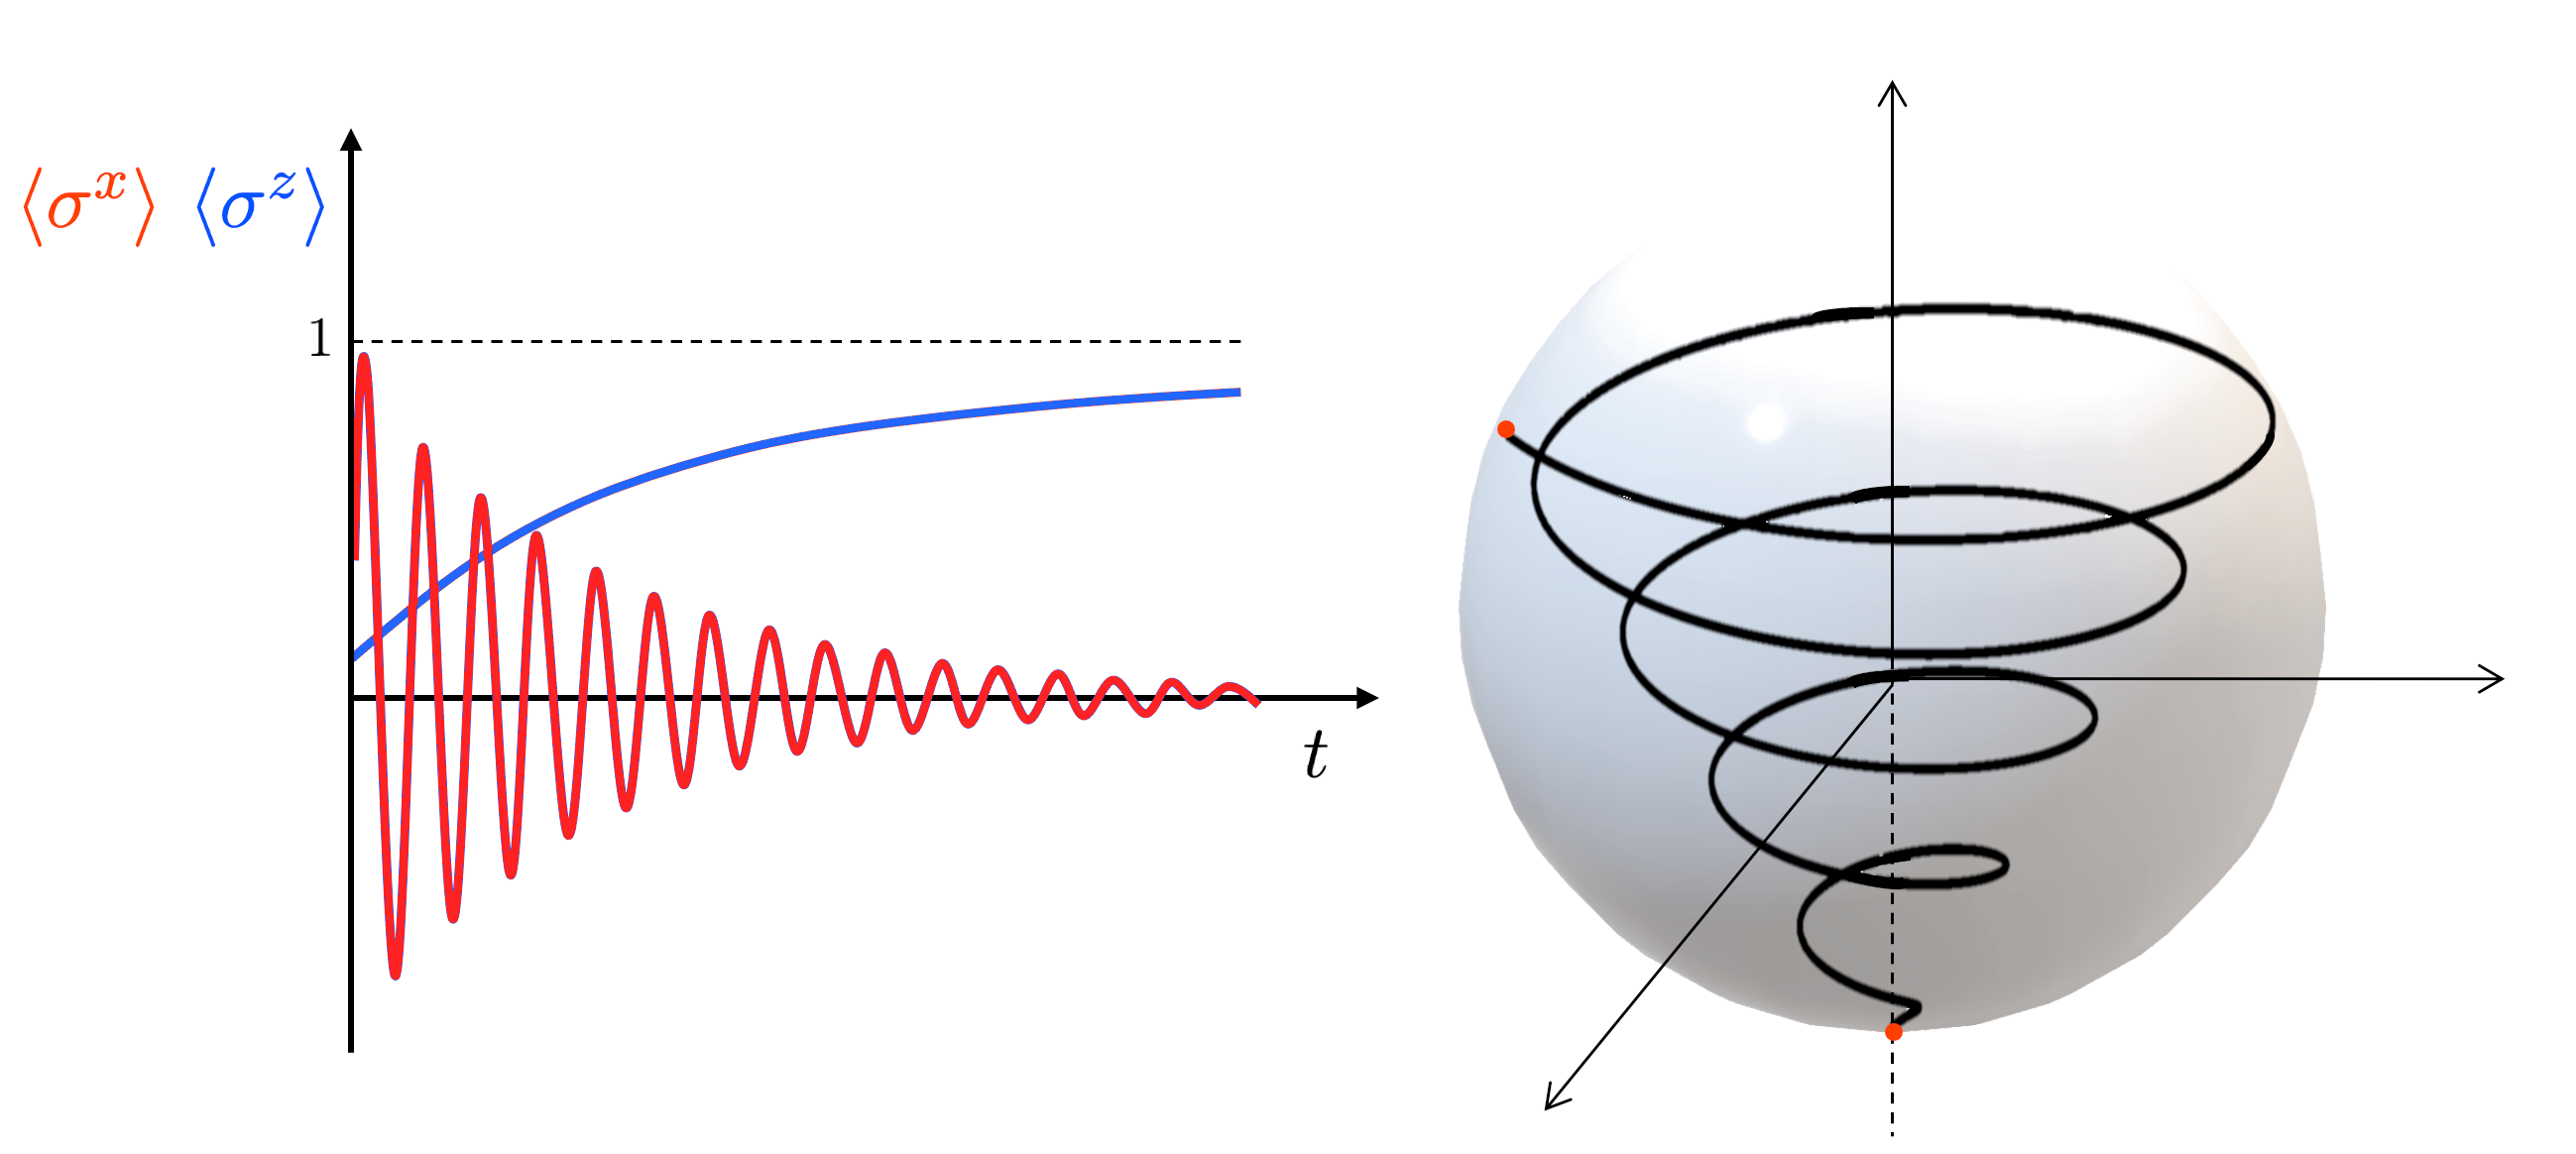
\includegraphics[width=0.87\linewidth]{images/Decay.png}
    \caption{Decay of a mixed state after the action of the Lindblad operator $L = \ket{g}\bra{e}$; the oscillation frequency of $\langle \sigma^x \rangle$ is equal to $\omega$, while the exponential decay of $\langle \sigma^z \rangle$ it is characterized by a frequency $\gamma$ (the same of $L$).}
    \label{fig:decay}
\end{figure}

Moreover, in the limit $t \to \infty$ the matrix operator becomes 
\begin{align*}
    \rho_\infty = \begin{pmatrix} 1 & 0 \\ 0 & 0 \end{pmatrix} = \ket{g}\bra{g}
\end{align*}
and it describes a steady state.
\end{tcolorbox}



\begin{tcolorbox} [breakable, enhanced]
\textbf{Dephasing (first part)} \\ 
Consider a two-level system descrived by the Hamiltonian 
\begin{align*}
    H = \hbar \omega \ket{e}\bra{e} = \hbar \omega \begin{pmatrix} 0 & 0 \\ 0 & 1 \end{pmatrix} 
\end{align*}
and take a single Lindblad operator $L = \ket{e}\bra{e}$. Therefore $\gamma$ is equal to the rate associated to the phase flip of the state. Also in this case, one can start from the generic expression of the density operator (\ref{eq:gen_rho}) in order to rewrite equation (\ref{eq:Lindblad}):
\begin{align*}
    \begin{pmatrix} \dot{a}(t) & \dot{b}(t) \\ \dot{b}^*(t) & \dot{c}(t) \end{pmatrix} =&~ i \omega \begin{pmatrix} 0 & b(t) \\ b^*(t) & 0 \end{pmatrix} + \gamma \Bigg( \begin{pmatrix} 0 & 0 \\ 0 & c(t) \end{pmatrix} + \\
    & - \frac{1}{2} \begin{pmatrix} 0 & b(t) \\ 0 & c(t) \end{pmatrix} - \frac{1}{2} \begin{pmatrix} 0 & 0 \\ b^*(t) & c(t) \end{pmatrix} \Bigg)
\end{align*}
and to obtain the differential equations for $b(t)$ and $c(t)$
\begin{align*}
    \begin{cases}
    \dot{b}(t) = \displaystyle \left( i \omega - \dfrac{\gamma}{2}\right) b(t) \\
    \dot{c}(t) = 0 
    \end{cases}
\end{align*}
Therefore
\begin{align*}
    \rho(t) = \begin{pmatrix} 1-c_0 & b_0 \, e^{t(i\omega - \gamma/2)} \\ \text{c.c.} & c_0 \end{pmatrix},
\end{align*}
where $a_0$, $b_0$ in $c_0$ are the matrix elements at the initial time. Some expectation values can be evaluated:
\begin{align*}
    \langle \sigma^z \rangle &= a(t) - c(t) = 1 - 2 c_0 \qquad (\text{conserved quantity}), \\
    \langle \sigma^x \rangle &= b(t) + b^*(t) = e^{-\gamma t /2} \, \real{\left(b_0 \, e^{i \omega t }\right)} = e^{-\gamma t /2} b_0 \cos{(\omega t)}  \qquad (b_0 \in \mathbb{R}),
\end{align*}
while in the limit $t \to \infty$ the matrix operator becomes
\begin{align*}
    \rho_\infty = \begin{pmatrix} 1-c_0 & 0 \\ 0 & c_0 \end{pmatrix},
\end{align*}
which describes a non-unique steady state. 
\end{tcolorbox}

\begin{figure}[H]
\centering
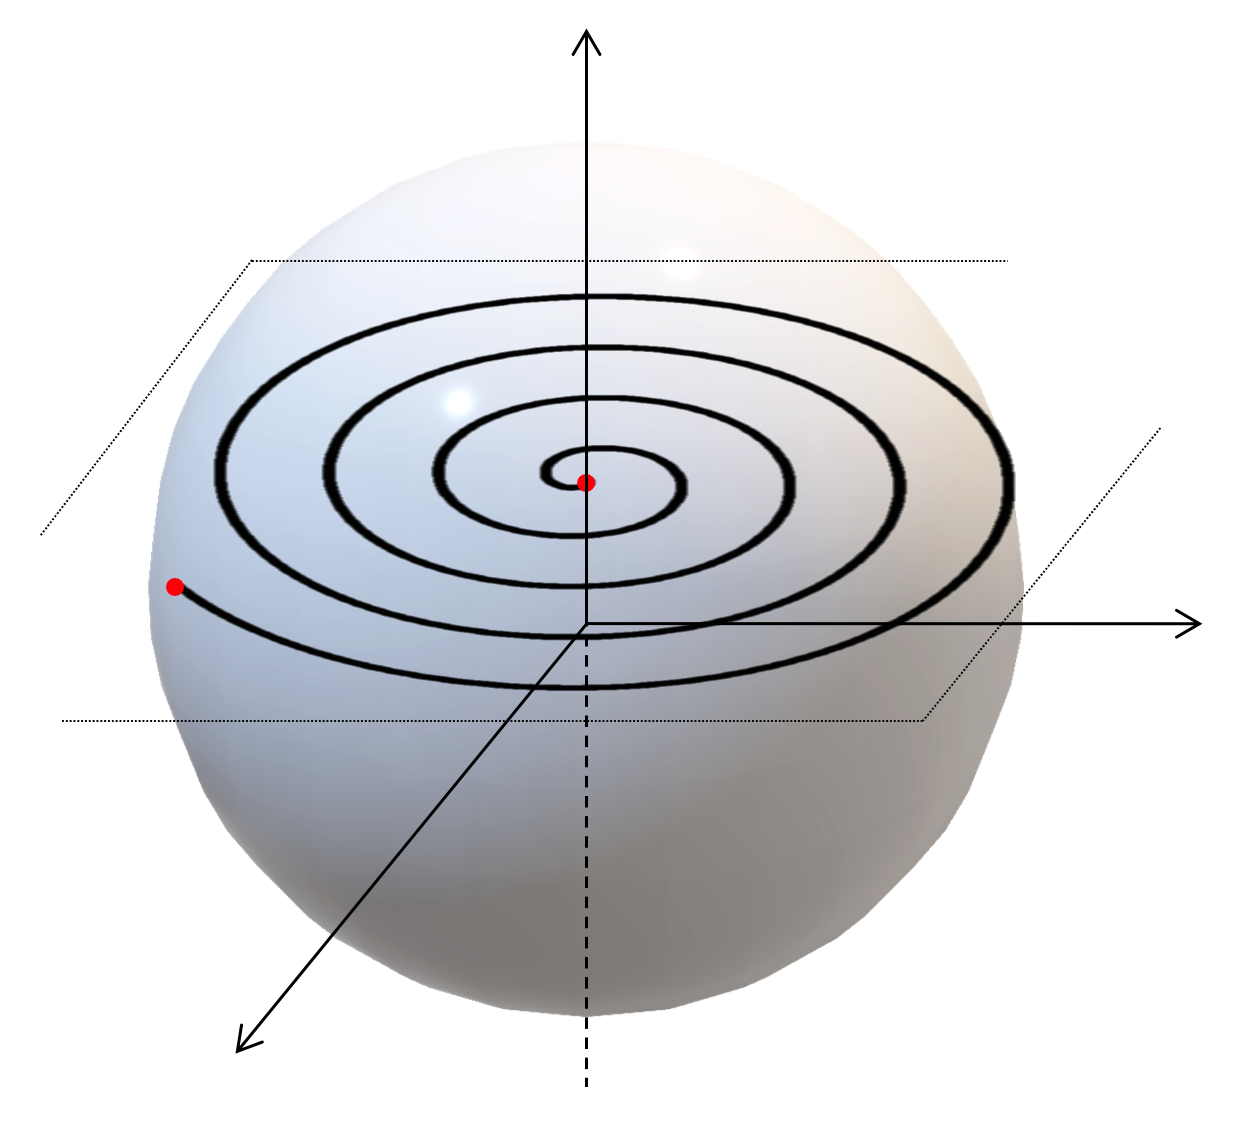
\includegraphics[width=0.47\linewidth]{images/Dephasing.png}
    \caption{Dephasing of a mixed state after the action of the Lindblad operator $L = \ket{e}\bra{e}$; the oscillation frequency of $\langle \sigma^x \rangle$ is equal to $\omega$.}
    \label{fig:dephasing}
\end{figure}

In both the presented examples, the entropy is not a precise indicator of the information of the system. Indeed, through explicit calculation, it is possible to show that in the second case $\mathcal{S}$ increases more with the respect to the first one, but the loss of information is reduced, since the evolution plane is known. 

\begin{tcolorbox} [breakable, enhanced]
\textbf{Dephasing (second part)} \\ 
Consider a two-level system described by the Hamiltonian
\begin{align*}
    H = \hbar \omega \ket{e}\bra{e} = \hbar \omega \begin{pmatrix} 0 & 0 \\ 0 & 1 \end{pmatrix} 
\end{align*}
and consider it subject to a classical noise (and not coupled to a bath). Therefore $\omega$ is a fixed random variable extracted from a probability distribution with probability density given by a Cauchy-Lorentzian distribution
\begin{align*}
    \frac{d p}{d \omega} = \frac{1}{\pi} \frac{\gamma}{(\omega - \omega_0)^2 + \gamma^2}. 
\end{align*}
With a procedure analogous to the one presented in the previous example, the density operator for a fixed valued of $\omega$ is
\begin{align*}
    \rho_\omega(t) = \begin{pmatrix} 1-c_0 & b_0 \, e^{i\omega t} \\ b_0^* \, e^{- i\omega t} & c_0 \end{pmatrix},
\end{align*}
while the one for the Hamiltonian ensemble is 
\begin{align*}
    \rho_\text{ensemble}(t) &= \int \rho_\omega(t) \, dp(\omega) = \bigintsss \begin{pmatrix} 1-c_0 & b_0 \, e^{i\omega t} \\ b_0^* \, e^{- i\omega t} & c_0 \end{pmatrix} \frac{dp}{d\omega} d\omega = \\
    &= \begin{pmatrix} 1-c_0 & b_0 \displaystyle \int e^{i\omega t} \dfrac{dp}{d\omega} d \omega \\ b_0^* \displaystyle \int e^{-i\omega t} \dfrac{dp}{d\omega} d \omega & c_0 \end{pmatrix} = \\
    &=  \begin{pmatrix} 1-c_0 & b_0 \, e^{(i\omega_0-\gamma) t} \\ \text{c.c.} & c_0 \end{pmatrix},
\end{align*}
where the last equation comes from 
\begin{align*}
    \int_{-\infty}^{+\infty} \frac{d \omega}{\pi} \frac{\gamma e^{i \omega t}}{(\omega - \omega_0)^2 + \gamma^2} = e^{i \omega_0 t - \gamma \abs{t}}.
\end{align*}
It is important to notice that the result for $\rho_\text{ensemble}$ is equivalent to the one obtained in the previous example for an open system coupled to a bath: Born-Markovian dynamics also models some forms of classical noise. 
\end{tcolorbox}

\subsection{Formal integration of the Lindblad Master equation}

The formal integration of the Lindblad Master equation can be performed by means of a \textit{vectorialization} procedure. In the first place, one can introduce the \textit{Liouvillian super-operator} (a super-operator is just an operator acting on an operator)
\begin{equation}
    \mathcal{L}(\rho) \equiv \frac{i}{\hbar} [\rho,H] + \sum_j \gamma_j \left( L_j \, \rho \,  L_j^\dagger - \frac{1}{2} \Bigl\{ L_j^\dagger L_j, \, \rho \Bigr\} \right),
    \label{eq:Liouvillian}
\end{equation}
and one can notice that equation (\ref{eq:Lindblad}) is equivalent to the Schr\"odinger equation, because $\mathcal{L}$ is a first order (in time) and linear operator ($\mathcal{L}(\rho_1 + \rho_2) = \mathcal{L}(\rho_1) + \mathcal{L}(\rho_2)$), and one is able to formally integrate it. In order to do this, some other steps are necessary and they constitute the \textit{Choi-Jamiolkowski isomorphism} (or vectorization). The latter can be captured by the relation
\begin{align}
    \ket{i}\bra{j} \quad \longrightarrow \quad \ket{j} \otimes \ket{i} \equiv \ket{ij}\rangle
    \label{eq:Choi}
\end{align}
and therefore one can think about an outer product (which has two indices) as being just a vector (with one index). In addition, using (\ref{eq:Choi}) the density matrix $\rho$ (with dimension dim$_H$ x dim$_H$) is transformed into the super-vector $\ket{\rho}\rangle$ (with dimension dim$^2_H$ x 1): 
\begin{align*}
        \rho = \sum_{i, \, j} \rho_{ij} \ket{i}\bra{j} \quad \longrightarrow \quad \ket{\rho}\rangle = \sum_{i, \, j} \rho_{ij} \ket{ij}\rangle.
\end{align*}
From a matrix point of view, this operation is the same as stacking columns of a matrix:
\begin{align}
    M = \begin{pmatrix} a & b \\ c & d \end{pmatrix}  \quad \longrightarrow \quad \ket{M}\rangle = \begin{pmatrix} a \\ b \\ c \\ d \end{pmatrix}.
    \label{eq:matrixtransf}
\end{align}
This trick is very useful due to two particular properties:
\begin{enumerate}
    \item The first one is related to the \textit{Hilbert-Schmidt inner product} (which satisfies all the properties of an inner product and therefore is analogous to $\braket{i}{j}$), defined as
    \begin{align*}
        \left( A,B\right)_{\mathcal{HS}} \equiv \langle \braket{A}{B} \rangle = \text{Tr}\left[ A^\dagger B \right].
    \end{align*}
    From this relation and (\ref{eq:matrixtransf}), one can intuitively guess that 
    \begin{align}
         \text{Tr}\left[ A^\dagger B \right] = \ket{A}\rangle^\dagger \ket{B}\rangle =  \langle \braket{A}{B} \rangle, 
         \label{eq:traceVect}
    \end{align}
    that is just the inner product between two vectors. 
    \item The second property is 
    \begin{align}
        \ket{A\, B\, C}\rangle = \left( C^t \otimes A \right) \ket{B}\rangle.
    \end{align}
    The usefulness of this relation lies in the fact that it provides a recipe to write super-operator products in the form of a big matrix times $\ket{{\rho}}\rangle$:
    \begin{align*}
        \ket{A{\rho}}\rangle = \ket{A \, {\rho} \, \mathbb{1}}\rangle = (\mathbb{1} \otimes A) \ket{{\rho}}\rangle 
    \end{align*}
\end{enumerate}
With these properties it is possible to rewrite the Liouvillian super-operator $\mathcal{L}$ as a super-matrix $\hat{\hat{\mathcal{L}}}$, indeed the two terms of (\ref{eq:Liouvillian}) become:
\begin{align*}
    \ket{\frac{i}{\hbar} [\rho,H]}\biggr\rangle &= -\frac{i}{\hbar} \left( \mathbb{1} \otimes H - H^t \otimes \mathbb{1} \right) \ket{\rho}\rangle,\\
    \ket{ L_j \, \rho \,  L_j^\dagger - \frac{1}{2} \Bigl\{ L_j^\dagger L_j, \, \rho \Bigr\} } \biggr\rangle &= \left( L_j^t \otimes L_j - \frac{1}{2} \mathbb{1} \otimes L_j^\dagger L_j - \frac{1}{2} (L_j^\dagger L_j)^t \otimes \mathbb{1} \right) \ket{\rho}\rangle.
\end{align*}
Therefore, the original Lindblad Master equation becomes 
\begin{align}
    \ket{\dot{\rho}}\rangle = \hat{\hat{\mathcal{L}}} \ket{{\rho}}\rangle
    \label{eq:LindbladVect}
\end{align}
with 
\begin{align}
    \hat{\hat{\mathcal{L}}} = -\frac{i}{\hbar} \left( \mathbb{1} \otimes H - H^t \otimes \mathbb{1} \right) + \sum_j \gamma_j \left( L_j^t \otimes L_j - \frac{1}{2} \mathbb{1} \otimes L_j^\dagger L_j - \frac{1}{2} (L_j^\dagger L_j)^t \otimes \mathbb{1} \right) 
\end{align}
Equation (\ref{eq:LindbladVect}) is similar to the Schr\"odinger equation, therefore one can suppose a solution of the form
\begin{align}
    \ket{\rho(t)}\rangle = \exp{\hat{\hat{\mathcal{L}}}t} \ket{\rho_0}\rangle. 
\end{align}
However $\hat{\hat{\mathcal{L}}}$ is not Hermitian and hence it is not guaranteed that it can be diagonalized. Nevertheless, if it is possible to find a matrix transformation $X$ such that $\hat{\hat{\mathcal{L}}} = X D X^\dagger$ (with $D$ diagonal matrix), then the solution is 
\begin{align}
    \ket{\rho(t)}\rangle = X e^{Dt} X^{-1}\ket{\rho_0}\rangle. 
\end{align}
Some final comments can be done:
\begin{itemize}
    \item The matrix $X$ is not an orthonormal matrix and its elements can be complex; in order to consider only physical solutions (in this case these that do not explodes exponentially), one must impose that $\forall d_j \in D$, $\real{(d_j)} \leq 0$.
    \item The steady state is
    \begin{align*}
        \ket{\dot{\rho}_{SS}}\rangle = 0 \qquad \Longleftrightarrow \qquad \hat{\hat{\mathcal{L}}} \ket{{\rho_{SS}}}\rangle = 0
    \end{align*}
    and hence $\ket{{\rho_{SS}}}\rangle$ must be in the kernel of $\hat{\hat{\mathcal{L}}}$. 
    \item Not all the eigenvectors are density matrix with unitary trace. In order to verify this, notice that the solutions of the eigen(super-)value equation $\hat{\hat{\mathcal{L}}} \ket{\Bar{\rho}}\rangle = \lambda \ket{\Bar{\rho}}\rangle$ associated to (\ref{eq:LindbladVect}) can be written as $\ket{\Bar{\rho}(t)}\rangle = e^{\lambda t} \ket{\Bar{\rho}_0}\rangle$; moreover, equation (\ref{eq:LindbladVect}) preserves the norm, indeed form (\ref{eq:traceVect})
    \begin{align*}
        \text{Tr}[\rho] = \text{Tr}[\mathbb{1} \, \rho] =  \text{Tr}[\mathbb{1}^\dagger \rho] = \langle \braket{\mathbb{1}}{\rho}\rangle = 1,
    \end{align*}
    therefore, if $\real{(\lambda)} < 0$, 
    \begin{align*}
        \text{Tr}[{\Bar{\rho}}_0] = \text{Tr}[\Bar{\rho}] = e^{\lambda t} \text{Tr}[{\Bar{\rho}_0}] \qquad \implies \qquad \text{Tr}[{\Bar{\rho}}] =  \text{Tr}[\Bar{\rho}] = 0.
    \end{align*}
    This means that all decaying eigen(super-)vectors are traceless and are not density matrices. 
\end{itemize}
